%%%% CAPÍTULO 4 - RESULTADOS E DISCUSSuO

\chapter{Results}\label{cap:resultados}

\section{Model Accuracy}

The most lightweight models were the preferred ones considering our edge device capabilities,
as they offer better inference time performance. 
However, we were also looking for the most optimal accuracy and loss metrics, 
therefore the models were evaluated with test images, which were never introduced to the models
during training, to make sure that they were efficient on the what they are ultimately supposed to do, 
which is to detect products.

Figures \ref{fig:singleclassification} and \ref{fig:multiclassification} show examples of 
Single and Multi label classification examples respectively.

% \begin{figure}[H]
% 	\caption[Single-Label Classification Examples]{Single-Label Classification Examples}
%     \begin{subfigure}{0.5\textwidth}
%         \centering
%         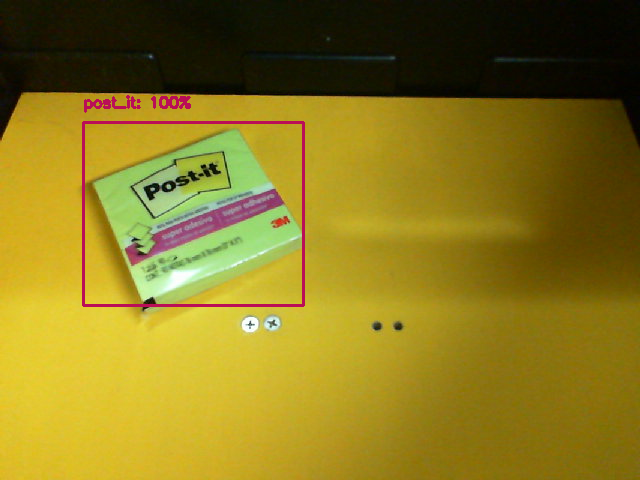
\includegraphics[width=.95\textwidth]{./images/singlelabel-classification-1.png}
%         \caption{}
%     \end{subfigure}
%     \begin{subfigure}{0.5\textwidth}
%         \centering
%         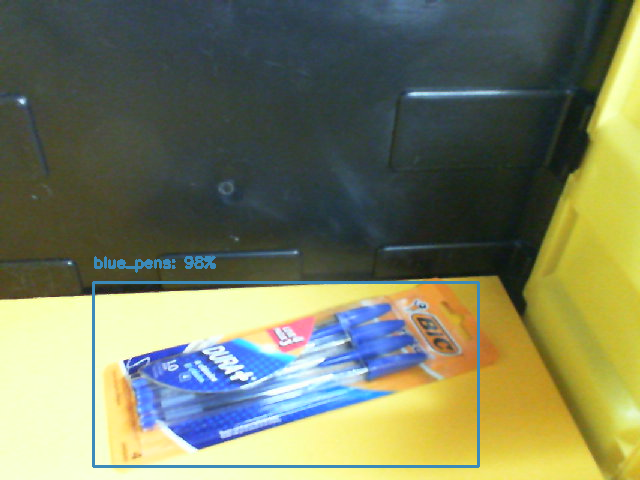
\includegraphics[width=.95\textwidth]{./images/singlelabel-classification-2.png}
%         \caption{}
%     \end{subfigure}
% 	\fonte{}
%     \label{fig:singleclassification}
% \end{figure}
% \begin{figure}[H]
%     \begin{subfigure}{0.5\textwidth}
%         \centering
%         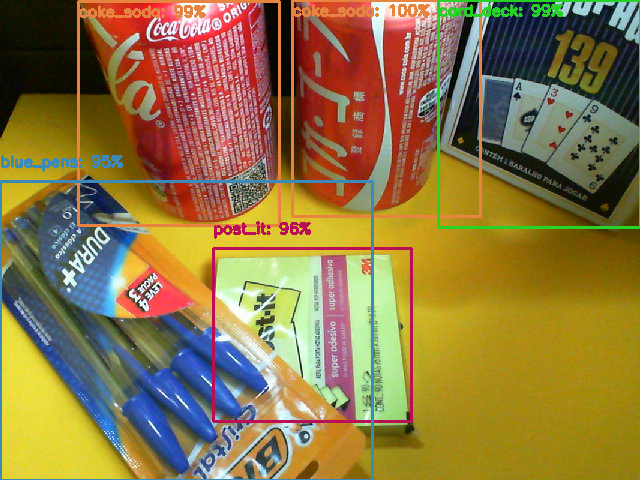
\includegraphics[width=.95\textwidth]{./images/multilabel-classification-1.png}
%         \caption{}
%     \end{subfigure}
%     \begin{subfigure}{0.5\textwidth}
%         \centering
%         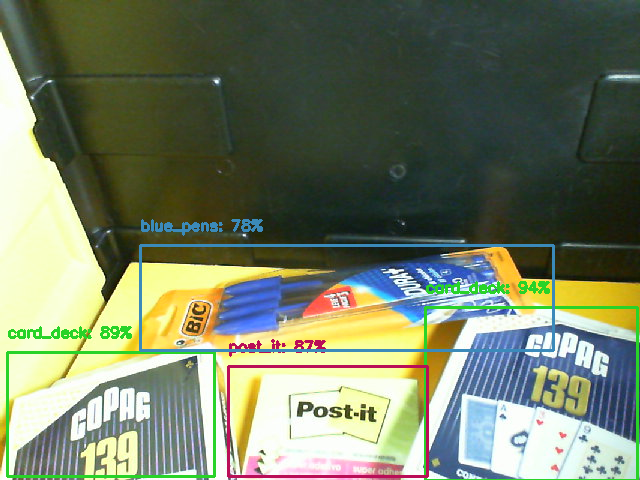
\includegraphics[width=.95\textwidth]{./images/multilabel-classification-2.png}
%         \caption{}
%     \end{subfigure}
% 	\caption[Multi-Label Classification Examples]{Multi-Label Classification Examples}
% 	\fonte{}
%     \label{fig:multiclassification}
% \end{figure}

The accuracy metrics were also inferred in our Test data set by using the TensorFlow Lite's 
Object Detector \textit{evaluate} method\footnote{https://www.tensorflow.org/lite/api\_docs/python/tflite\_model\_maker/object\_detector/ObjectDetector\#evaluate}
for all different model configurations that were applied. 
The main evaluation metrics for the models considered for our product, which were the ones based 
in the EfficientDet-D0, D1 and D2 architectures -- as the D3 and D4 architectures were too 
computationally expensive for our device -- are listed in Table 4. 

The numbers exhibited in the table consist of the classification Average Precision 
(\sigla{AP}{Average Precision}), which measures the percentage of correctly labeled 
predictions amongst all predictions; the AP with an IoU of 50\%, which means that
there is at least 50\% of overlap between the predicted and the actual bounding boxes; 
the AP with an IoU of 75\%; and the individual classification APs for each label that 
was forecasted. 

% \begin{table}[H]
% 	\label{tab:modelPerformance}
% 	\centering
% 	\caption[Test Evaluation Metrics for the Different Strategies and Models Applied for Inference]{Test Evaluation Metrics for the Different Strategies and Models Applied for Inference}
% 	\begin{adjustbox}{width=1\textwidth}
% 	\begin{tabular}{c|c|c|c|c|c|c|c|c|c|c}
% 		\hline 
% 		Architecture & Preprocessing Strategy & Training Strategy & AP & AP 50 IoU & AP 75 IoU & AP (post\_it) & AP (guarana) & AP (coke) & AP (card\_deck) & AP (blue\_pens) \\
% 		\hline
%         Efficientdet\-D0 & Resizing & Transfer Learning & \texttt{0.527} & \texttt{0.700} & \texttt{0.644} & \texttt{0.521} & \texttt{0.443} & \texttt{0.685} & \texttt{0.490} & \texttt{0.497} \\
% 		Efficientdet\-D1 & Resizing & Transfer Learning & \texttt{0.623} & \texttt{0.786} & \texttt{0.740} & \texttt{0.409} & \texttt{0.639} & \texttt{0.812} & \texttt{0.670} & \texttt{0.588} \\
% 		Efficientdet\-D2 & Resizing & Transfer Learning & \texttt{0.653} & \texttt{0.799} & \texttt{0.774} & \texttt{0.587} & \texttt{0.659} & \texttt{0.825} & \texttt{0.669} & \texttt{0.524} \\
% 		Efficientdet\-D0 & Resizing & Whole & \texttt{0.813} & \texttt{0.978} & \texttt{0.906} & \texttt{0.752} & \texttt{0.765} & \texttt{0.891} & \texttt{0.921} & \texttt{0.736} \\
% 		Efficientdet\-D1 & Resizing & Whole & \texttt{0.802} & \texttt{0.939} & \texttt{0.875} & \texttt{0.719} & \texttt{0.675} & \texttt{0.903} & \texttt{0.928} & \texttt{0.785} \\
% 		\textbf{Efficientdet\-D2} & \textbf{Resizing} & \textbf{Whole} & \textbf{0.826} & \textbf{0.967} & \textbf{0.922} & \textbf{0.763} & \textbf{0.776} & \textbf{0.910} & \textbf{0.895} & \textbf{0.784} \\
% 		Efficientdet\-D0 & Cropping & Transfer Learning & \texttt{0.490} & \texttt{0.668} & \texttt{0.592} & \texttt{0.357} & \texttt{0.422} & \texttt{0.595} & \texttt{0.633} & \texttt{0.443} \\
% 		Efficientdet\-D1 & Cropping & Transfer Learning & \texttt{0.580} & \texttt{0.730} & \texttt{0.686} & \texttt{0.312} & \texttt{0.605} & \texttt{0.716} & \texttt{0.736} & \texttt{0.531} \\
% 		Efficientdet\-D2 & Cropping & Transfer Learning & \texttt{0.562} & \texttt{0.722} & \texttt{0.699} & \texttt{0.463} & \texttt{0.569} & \texttt{0.576} & \texttt{0.661} & \texttt{0.539} \\
% 		Efficientdet\-D0 & Cropping & Whole & \texttt{0.832} & \texttt{0.954} & \texttt{0.934} & \texttt{0.869} & \texttt{0.854} & \texttt{0.717} & \texttt{0.922} & \texttt{0.800} \\
% 		Efficientdet\-D1 & Cropping & Whole & \texttt{0.792} & \texttt{0.897} & \texttt{0.880} & \texttt{0.823} & \texttt{0.763} & \texttt{0.586} & \texttt{0.933} & \texttt{0.852} \\
% 		Efficientdet\-D2 & Cropping & Whole & \texttt{0.803} & \texttt{0.923} & \texttt{0.893} & \texttt{0.795} & \texttt{0.808} & \texttt{0.631} & \texttt{0.941} & \texttt{0.840} \\
% 		\hline 
% 	\end{tabular}
% 	\end{adjustbox}
% 	\label{tab:modelPerformance}
% 	\fonte{}
% \end{table}

We could clearly see that, while the Transfer Learning models were much faster to train,
in our particular case, the Whole-trained models outperformed them. This could be 
due to the fact that our pictures and objects are different from the
ones that are present in the COCO-2017 dataset; or because a custom feature extractor- 
with custom hidden layer weights and biases- could have better performance with our pictures. 
In terms of the architectures, as expected, the D2 architecture offered more robust results, specially
amongst the models that applied resizing as a preprocessing strategy. 

We could not see much superior metrics for the models that used cropping for the images preprocessing, 
and that might be because most of the bounding boxes ended up being cropped as well and, with that, we lost
a portion of valuable label data. Altough the EfficientDet-D0 model that was Whole-Trained with Cropped images
had a comparable performance in our Test Data evaluation, considering the end-to-end usability tests that we executed 
with the assembled prototype and the overall better performance presented by the D2 architecture, as shown in
figure \ref{fig:yoloefficientdet}, we selected the EfficientDet-D2 model that was Whole-Trained with Resized
images as our champion model.

The loss (error) metrics during training were also computed for our Train and Validation sets during the 
200 epochs that were used for training our models using batches of 16 images, for all different 
settings that were employed to train them. We can clearly state that the model showed significant
improvement as the epochs progressed, and maybe more epochs would even have brought greater performance,
as the weights would have been even more fine-tuned. The trade-off, though, is that it would have 
taken more time and computer power to train the models.
In Figure \ref{fig:training}, you can find the Classification Loss chart for our three top models of choice, which were
the EfficientDet-D0, D1 and D2, whole-trained and that used resizing as a preprocessing strategy.

% \begin{figure}[H]
% 	\centering
%     \begin{subfigure}{0.65\textwidth}
%         \centering
%         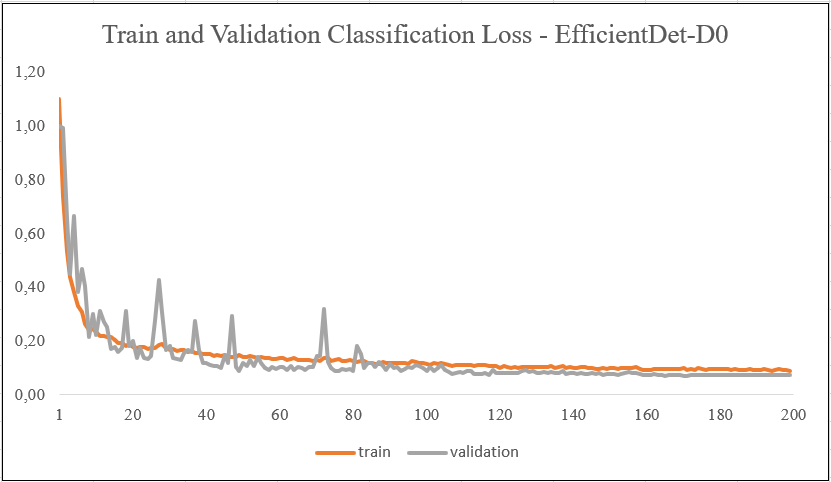
\includegraphics[width=1\textwidth]{./images/efficientdet-d0-resized-whole-loss.png}
%         \caption{}
%     \end{subfigure}
%     \begin{subfigure}{0.65\textwidth}
%         \centering
%         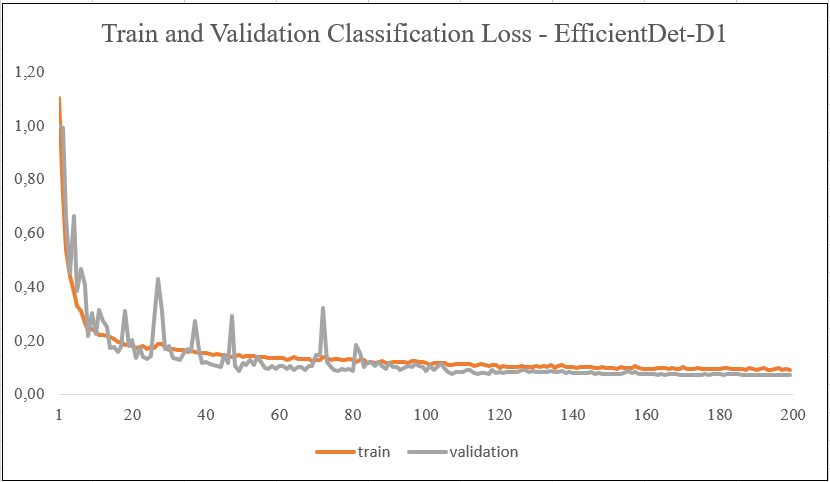
\includegraphics[width=1\textwidth]{./images/efficientdet-d1-resized-whole-loss.png}
%         \caption{}
%     \end{subfigure}
%     \begin{subfigure}{0.65\textwidth}
%         \centering
%         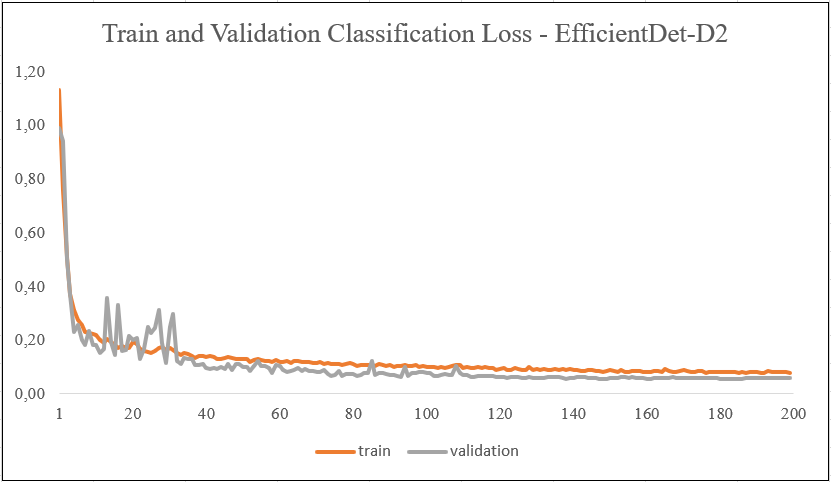
\includegraphics[width=1\textwidth]{./images/efficientdet-d2-resized-whole-loss.png}
%         \caption{}
%     \end{subfigure}
% 	\caption[Train and Validation Classification Loss for the EfficientDet Models that 
% 		was whole-trained and took resized images as an input]{Train and Validation Classification Loss 
% 		for the EfficientDet Models that was whole-trained and took resized images as an input}
% 	\fonte{}
%     \label{fig:training}
% \end{figure}

Note that those spikes in the loss values are probably due to the batch size, as it could be 
that in specific batches of 16 images the model was not fully prepared to predict the labels
in those images. Using a larger batch would likely solve it, however it would also take more RAM
memory consumption. 

Finally, to improve inference time performance, we also compiled our TensorFlow Lite models for 
usage with an Edge TPU, which further reduced our inference times. 

\begin{table}[H]
	\centering
	\caption[Inference Performance Metrics with and without the TPU]{Inference Performance Metrics with and without the TPU}
	\begin{adjustbox}{width=1\textwidth}
	\label{tab:modelPerformance}
	\begin{tabular}{c|c|c|c|c}
		\hline 
		Model & FPS without the TPU & FPS using the TPU & CPU Ops using the TPU & TPU Ops using the TPU\\
		\hline
        Efficientdet-D0 Whole-Trained on Resized Images & \texttt{3.69} & \texttt{6.87} & \texttt{3} & \texttt{264}\\
		Efficientdet-D1 Whole-Trained on Resized Images & \texttt{2.09} & \texttt{5.14} & \texttt{131} & \texttt{191}\\
		Efficientdet-D2 Whole-Trained on Resized Images & \texttt{1.36} & \texttt{3.50} & \texttt{131} & \texttt{226}\\ 
		\hline 
	\end{tabular}
	\end{adjustbox}
	\fonte{Own work}
\end{table}

Figure \ref{fig:framecount} displays an example frame from the camera feed displaying the 
current FPS count.

\begin{figure}[H]
	\centering
    \caption[Frame from camera feed with FPS count]{Frame from camera feed with FPS count}
	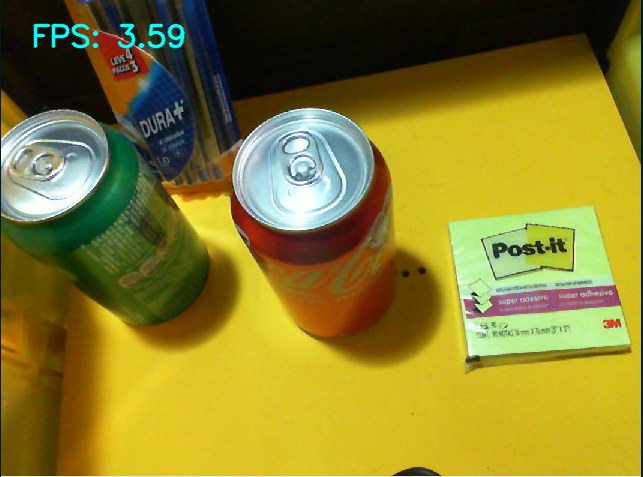
\includegraphics[width=0.5\textwidth]{./images/frameratemeasurement.png}
    \label{fig:framecount}
    \fonte{}
\end{figure}

The inference speed has thoroughly improved - about 50\% on average - resulting
in a greater capability to process more Frames Per Second. When we look at the
number of CPU and TPU Operations, though, what we would expect when using the
TPU is that most Operations happen on the TPU side, however this behavior could
only be seen in the EfficientDet-D0 model. Part of it is because the
EfficientDet-D0 model has a simpler architecture, but it could also be due to
the conversion of the model for usage with the TPU or to the limited capacity
of the TPU device that was used. For instance, Google suggests using two TPU
cores for the EfficientDet-D2
model\footnote{https://www.tensorflow.org/lite/models/modify/model\_maker/object\_detection},
because the tensors are too large to fit in the chip's memory.

Overall, after considering the tradeoff between precision and performance, we
have decided to use the EfficientDet-D2 model since its performance when paired
with the Coral TPU was more than enough for our purposes (around 4 FPS) and had
the best precision, improving the overall experience of the prototype.

\section{Power Consumption}

For estimating the overall power consumption, a commercial wattmeter was used
to observe the total power required by the power adapter used, as shown in
Figure \ref{fig:wattmeter}.

\begin{figure}[H]
	\centering
	\caption[Power consumption measurement using a wattmeter]{Power consumption measurement using a wattmeter}
    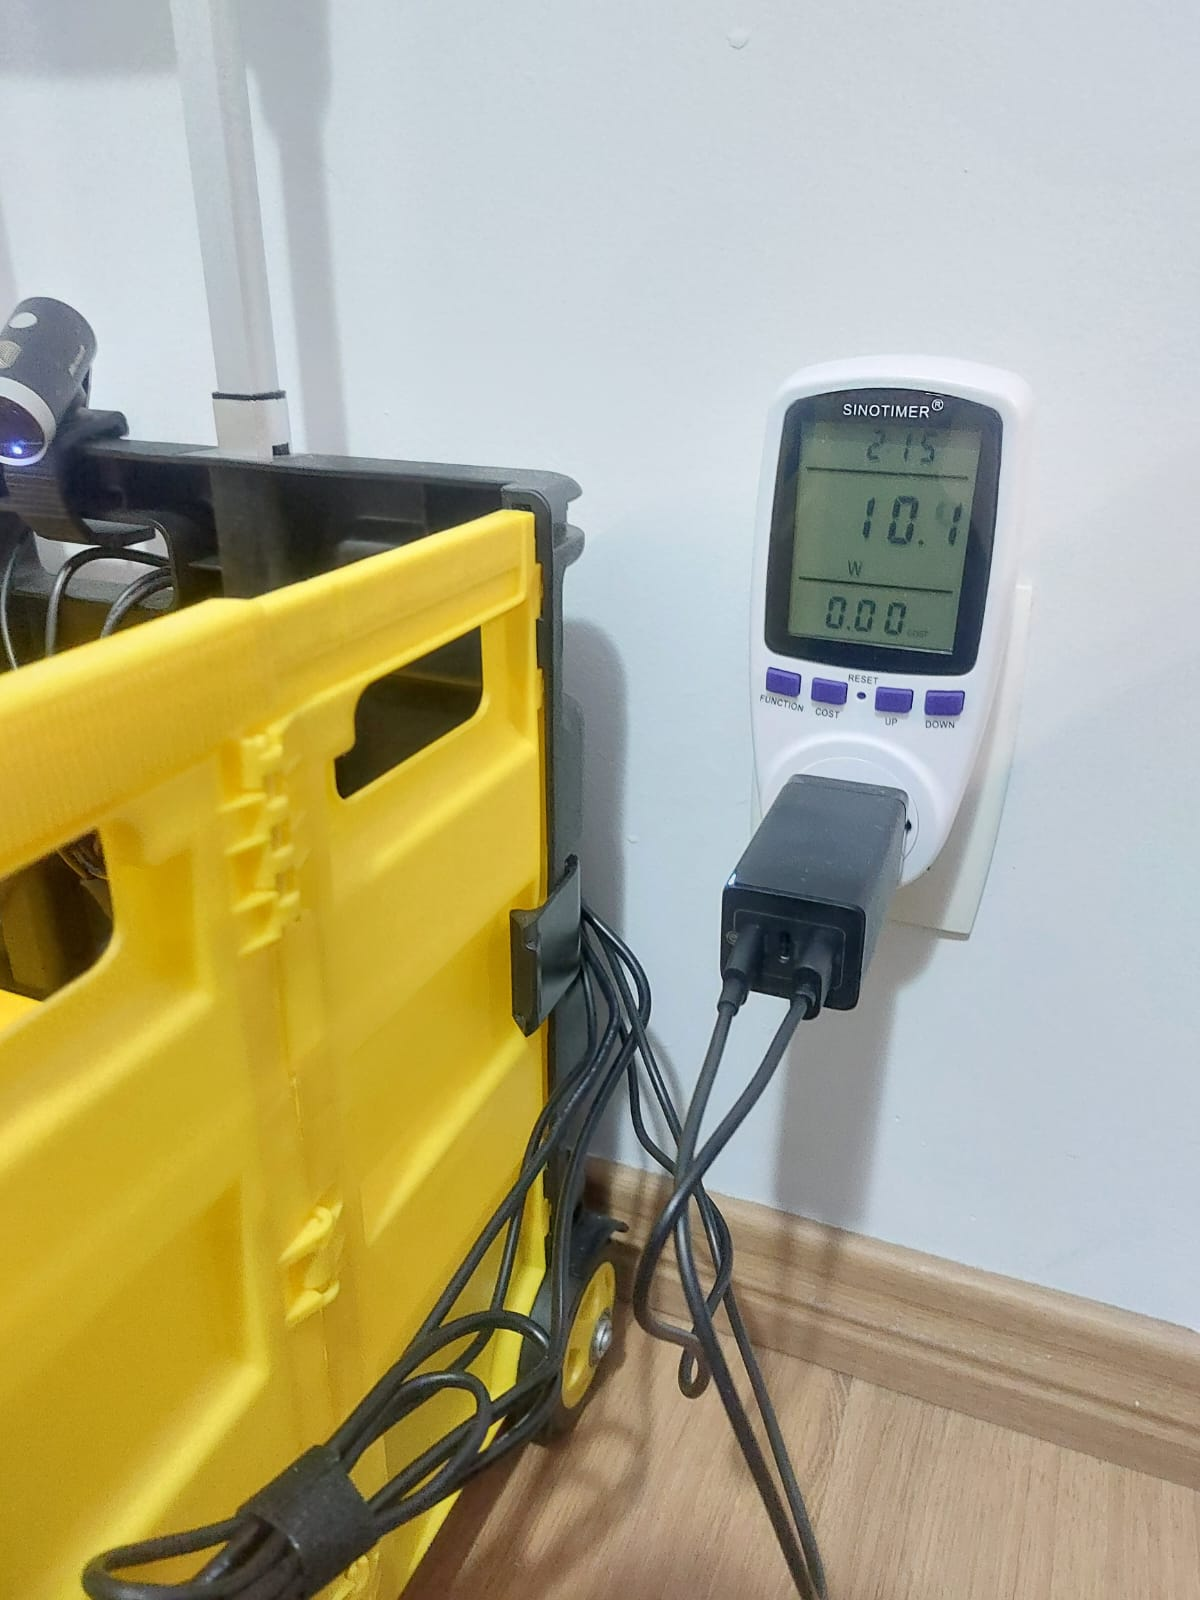
\includegraphics[width=0.5\textwidth]{./images/powerconsumption.jpeg}
	\fonte{}
    \label{fig:wattmeter}
\end{figure}

During our tests, we have observed an average consumption of \textbf{10,4W}
when running the all the software and hardware components of the prototype
through an external power adapter. 

The tests were performed on a 220V power line using the following equipment:
\begin{itemize}
    \item Sinotimer DDS108 Digital Wattmeter
    \item Baseus Quick Charger GaN 65W
\end{itemize}

Since both of these products do not have detailed accuracy and efficiency data
available, we estimate an overall 10\% margin of error considering their
construction \cite{Chen2017}. 

With that, we can assume that the actual power draw is between 9,4W and 11,4W.
Considering a desired  battery life of 24 hours, it would require a battery of
about 240 Wh, which can be found commercially and would not impose a
insurmountable practical barrier.

\section{Cost}

One of the important aspects when developing a marketable product is its \textbf{cost}.

A more detailed overview of the items and their costs is shown on Table \ref{tbl:cost}.

\begin{table}[H]
	\centering
	\label{tab:correlacao}
    \caption[Items used on the prototype and their approximate retail cost in Brazil as of October 2022]{Items used on the prototype and their retail cost in October 2022}
	\begin{tabular}{c c c}
		\hline 
        Item & Quantity & Cost per item (BRL/USD) \\
		\hline
        Raspberry Pi 4 8GB Board &  1 & R\$ 1072,40 / US\$ 201,94 \\
        Coral Edge TPU &  1 & R\$ 318,51 / US\$ 59,99 \\
        HX711 with breakout board &  1  & R\$ 2,55 / US\$ 0,48 \\
        10Kg Load Cell & 1 & R\$ 6,89 / US\$ 1,30 \\
        MDF Board &  2  & R\$ 10,00 / US\$ 1,89 \\
        Mounting hardware (screws, bolts and nuts) &  1  & R\$ 5,00 / US\$ 0,94 \\
        Foldable utility cart &  1  & R\$ 125,00 / US\$ 23,60 \\
        Webcam &  1  & R\$ 100,00 / US\$ 18,88 \\
		\hline 
        & Total cost & R\$ 1650,35 / US\$ 310,91 \\
        \hline
	\end{tabular}
	\fonte{}
    \label{tbl:cost}
\end{table}

Of course, the developed prototype does not include all the necessary hardware
and software structure to deliver a successful product, but still it might show that at a
fundamental level, the cost of such a solution might not reach the costs that
current smart carts in the market sell for\footnote{The Nextop cart shown on the
introduction currently retails for R\$ 120.000}.

Therefore, it might be possible to conclude that most of the retail cost of the
existing smart carts is not composed of the production and infrastructure costs
but from the required repayment of the research and development costs that such
a product demand.

\section{Challenges and future work}

As one of the expected outcomes of our work, we have been able to identify
several practical challenges that would need to be worked on for a marketable
product and will be discussed in the next sections.

\subsection{Extending the model for new products}
In a supermarket use case, we expect that products will need to be added or
removed from detection model on a regular basis. That becomes a challenge when
we consider the amount of data necessary to train the model used in the
developed prototype.

Considering that, an important next step on the development would be to work on
a model that can be easily extend to support new products without requiring too
much computational power for retraining.

\subsection{Deploying updates}

Considering the compute locality of the detection model used in the prototype,
which is the board embedded in the cart, deploying updates to the model to it
might become a challenge.

Changing the compute locality to  a Cloud infrastructure \cite{Aws2022} might
allow for easier deployment for updates but that comes with a trade off in
terms of latency, since networks calls would be required, and that can become
detrimental in such a real-time based product.

Investigating that trade off or even developing a solution for easy deployment
of model updates is another import development to be worked in the future. 

\subsection{Batteries and charging}

Another challenge identified for creating a viable product is to develop and
energy efficient solution that is capable of running on a reasonable battery
for at least an entire day.

As described in the testing section, the prototype is already capable of being
deployed with a reasonable commercial battery but we believe that there are
still margin for improvement.

Evidently, it is possible to include a battery with bigger capacity to the
product to provide better battery life but that comes with the trade off of
additional weight and cost, undesired characteristics from the end user and
grosser perspective respectively.

Additionally, it would be important to developed a practical mechanism to allow
the carts to be charged such as a docking mechanism or even by wireless
charging \cite{Treffers2015}, reducing the maintenance effort from the grocery's
perspective. 

\subsection{Loss Prevention}

As our research has shown, loss prevention is a key feature of a smart cart, specially in the Brazilian context
\cite{Nextop2022}.

In such scenario, it would be important to work on possible extra features that
would give the grosser the extra confidence to deploy the cart to his/her retail
chain.

\subsection{Improving accuracy and reliability}

Related to the subsection above, improving the accuracy and reliability of the
overall system is key not just for loss prevention but to provide a great user
experience. We believe that a sub par experience will eventually lead to disuse
and therefore our objective would be to achieve a \textit{transparent}
experience, where the user might even forget about all the technological feat
that allows the cart to function.
